\documentclass[10pt]{article}

% Encoding & fonts
\usepackage[T1]{fontenc}
\usepackage[utf8]{inputenc}
\usepackage{lmodern}

\usepackage{graphicx}
\usepackage{booktabs}
\usepackage{enumitem}
\usepackage{amsmath, amssymb}
\usepackage[a4paper, top=1.6cm, bottom=1.6cm, left=1.8cm, right=1.8cm]{geometry}
\usepackage{tikz}
\usetikzlibrary{shapes.geometric, arrows.meta, positioning, shadows, calc, fit, backgrounds}
\usepackage{xcolor}
\usepackage{caption}
\captionsetup{font=footnotesize, skip=3pt}

% Custom colors
\definecolor{scenarioBlue}{RGB}{52, 152, 219}
\definecolor{milpRed}{RGB}{231, 76, 60}
\definecolor{graphGreen}{RGB}{46, 204, 113}
\definecolor{encoderPurple}{RGB}{155, 89, 182}
\definecolor{ebmOrange}{RGB}{243, 156, 18}
\definecolor{samplerTeal}{RGB}{26, 188, 156}
\definecolor{decoderPink}{RGB}{233, 30, 99}
\definecolor{lpworkerBrown}{RGB}{121, 85, 72}
\definecolor{evalGray}{RGB}{96, 125, 139}

% Bibliography
\usepackage[round,authoryear]{natbib}
\let\parencite\citep

% Hyperlinks
\usepackage[hidelinks]{hyperref}

% Compact sections
\usepackage{titlesec}
\titlespacing*{\section}{0pt}{6pt}{3pt}
\titlespacing*{\paragraph}{0pt}{3pt}{3pt}

% Compact title
\makeatletter
\renewcommand{\maketitle}{%
  \begin{center}
    {\large\bfseries \@title \par}
    \vspace{2pt}
    {\normalsize \@author \par}
  \end{center}
  \vspace{-6pt}
}
\makeatother


\title{Coordinating Multilayer Power System Flexibility:\\
A Hybrid MILP--GNN--EBM Framework\,---\,Extended Abstract}

\author{Th\'eotime Coudray\textsuperscript{*} \quad St\'ephane Goutte\textsuperscript{*}\\[1pt]
{\small \textsuperscript{*}Universit\'e de Versailles Saint-Quentin-en-Yvelines (UVSQ), UMI SOURCE}}
\date{}

\begin{document}
\maketitle

% ============================================================
\section{Context and Motivation}

The energy transition demands flexibility coordination across multiple spatial layers and temporal scales. Operators increasingly need \emph{interactive scenario exploration}---evaluating thousands of what-if cases spanning extreme weather, topology changes, and new flexibility portfolios---rather than single-shot optimisation. Mixed-Integer Linear Programming (MILP) provides rigorous solutions but repeated solves become prohibitive as scenario count grows \citep{conejo_investment_2016, micheli_two-stage_2023}. GNN surrogates exploit topology for speed but often violate hard constraints \citep{liu_topology-aware_2023}. Energy-Based Models (EBMs) offer principled exploration of discrete spaces via gradient-guided sampling \citep{sun_annealed_2022}, yet have not been applied to multi-scale flexibility. We ask: \emph{Can a hybrid MILP--GNN--EBM methodology enable near-real-time flexibility scenario exploration---and remain effective as complexity increases?}

% ============================================================
\section{Methodology}

The proposed pipeline (Figure~\ref{fig:pipeline}) comprises five stages.
\textbf{(1)~Data Generation.} A synthetic scenario generator samples diverse power-system instances (4--160 zones) via Latin Hypercube Sampling and greedy $k$-centre selection, with an ex-ante \emph{criticality index} ranking each instance by physical stress and combinatorial hardness. A multi-layer MILP oracle then solves each scenario---jointly optimising thermal commitment, storage scheduling, demand-response activation, and cross-border exchanges---to produce ground-truth binary labels~$(u^*)$ and continuous dispatch~$(x^*)$.
\textbf{(2)~Representation Learning.} Each scenario is projected onto a heterogeneous temporal graph (5 node types, 11 edge types) encoding the containment hierarchy (nation$\to$region$\to$zone$\to$asset), transmission topology, weather influence, and inter-temporal couplings (SOC, ramping, DR cooldown). A Hierarchical Temporal Encoder (HTE), trained via self-supervised contrastive learning (InfoNCE with multi-lag positives) \emph{without MILP labels}, produces zone-level embeddings $h \in \mathbb{R}^{Z \times T \times 128}$ through bottom-up GATv2 spatial encoding, a nation-level Transformer for temporal reasoning, and top-down skip-connected decoding.
\textbf{(3)~Energy-Based Learning.} Conditioned on $h$, a GRU-based EBM learns an energy landscape over binary decisions $u \in \{0,1\}^{Z \times T \times 7}$. A logit-space Langevin sampler with temperature annealing generates diverse candidates. Training proceeds in two steps: contrastive divergence pre-training on gold (optimal) labels, then preference fine-tuning on silver labels using LP-evaluated cost rankings.
\textbf{(4)~Solution Reconstruction.} A greedy, EBM-guided feasibility decoder repairs binary candidates into physically consistent dispatch plans (power balance, storage dynamics, ramp limits). A two-stage LP worker then recovers the optimal continuous dispatch with progressive repair stages (hard-fix $\to$ targeted repair $\to$ full relaxation).
\textbf{(5)~Benchmarking.} The full pipeline is evaluated against the MILP oracle on 300 out-of-sample scenarios across three criticality families, measuring cost gap, speedup, feasibility, and LP stage distribution.

\begin{figure}[t]
\centering
\resizebox{0.92\textwidth}{!}{%
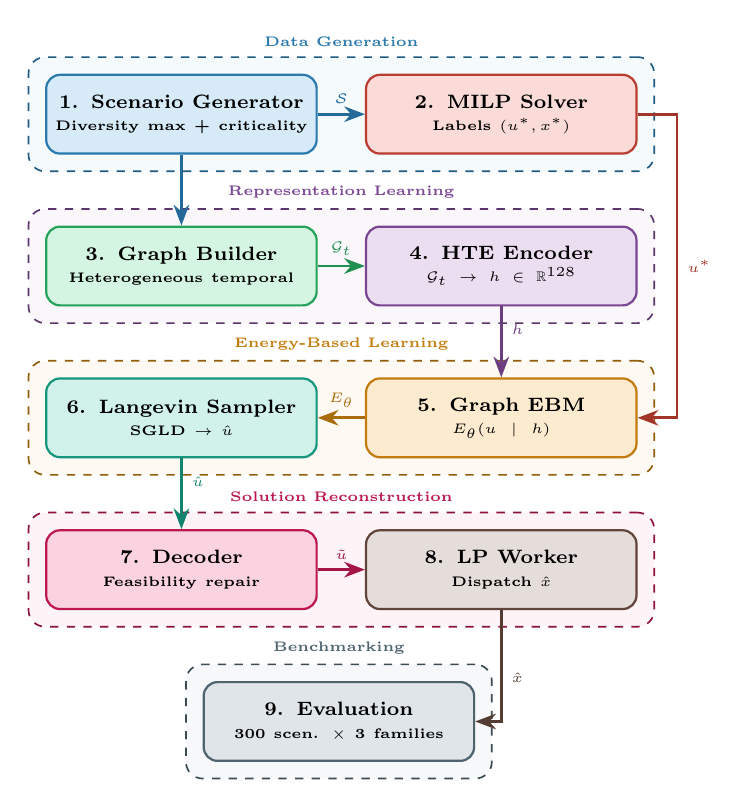
\begin{tikzpicture}[
    block/.style={
        rectangle, rounded corners=5pt, minimum width=3.4cm, minimum height=1cm,
        text centered, text width=3.2cm, font=\scriptsize\bfseries,
        draw=#1!80!black, fill=#1!20, line width=0.8pt,
        drop shadow={shadow xshift=0.4pt, shadow yshift=-0.4pt, opacity=0.15}
    },
    arrow/.style={->, >=Stealth, line width=1pt, draw=#1!70!black},
    annot/.style={font=\tiny\itshape, text=#1!70!black, align=center},
    groupbox/.style={draw=#1!60!black, fill=#1!5, rounded corners=6pt, line width=0.6pt, dashed}
]
\node[block=scenarioBlue] (generator) {\textbf{1. Scenario Generator}\\\tiny Diversity max + criticality};
\node[block=milpRed, right=0.6cm of generator] (milp) {\textbf{2. MILP Solver}\\\tiny Labels $(u^*, x^*)$};
\node[block=graphGreen, below=0.9cm of generator] (graphs) {\textbf{3. Graph Builder}\\\tiny Heterogeneous temporal};
\node[block=encoderPurple, right=0.6cm of graphs] (encoder) {\textbf{4. HTE Encoder}\\\tiny $\mathcal{G}_t \to h \in \mathbb{R}^{128}$};
\node[block=ebmOrange, below=0.9cm of encoder] (ebm) {\textbf{5. Graph EBM}\\\tiny $E_\theta(u \mid h)$};
\node[block=samplerTeal, left=0.6cm of ebm] (sampler) {\textbf{6. Langevin Sampler}\\\tiny SGLD $\to$ $\hat{u}$};
\node[block=decoderPink, below=0.9cm of sampler] (decoder) {\textbf{7. Decoder}\\\tiny Feasibility repair};
\node[block=lpworkerBrown, right=0.6cm of decoder] (lpworker) {\textbf{8. LP Worker}\\\tiny Dispatch $\hat{x}$};
\node[block=evalGray, below=0.9cm of decoder, xshift=2cm] (eval) {\textbf{9. Evaluation}\\\tiny 300 scen. $\times$ 3 families};
\draw[arrow=scenarioBlue] (generator.east) -- (milp.west) node[annot=scenarioBlue, midway, above] {$\mathcal{S}$};
\draw[arrow=scenarioBlue] (generator.south) -- (graphs.north);
\draw[arrow=milpRed] (milp.east) -- ++(0.5,0) |- (ebm.east) node[annot=milpRed, pos=0.25, right] {$u^*$};
\draw[arrow=graphGreen] (graphs.east) -- (encoder.west) node[annot=graphGreen, midway, above] {$\mathcal{G}_t$};
\draw[arrow=encoderPurple] (encoder.south) -- ++(0,-0.3cm) -| (ebm.north) node[annot=encoderPurple, pos=0.25, right] {$h$};
\draw[arrow=ebmOrange] (ebm.west) -- (sampler.east) node[annot=ebmOrange, midway, above] {$E_\theta$};
\draw[arrow=samplerTeal] (sampler.south) -- ++(0,-0.3cm) -| (decoder.north) node[annot=samplerTeal, pos=0.25, right] {$\hat{u}$};
\draw[arrow=decoderPink] (decoder.east) -- (lpworker.west) node[annot=decoderPink, midway, above] {$\tilde{u}$};
\draw[arrow=lpworkerBrown] (lpworker.south) -- ++(0,-0.3cm) |- (eval.east) node[annot=lpworkerBrown, pos=0.25, right] {$\hat{x}$};
\begin{scope}[on background layer]
    \node[groupbox=scenarioBlue, fit=(generator)(milp), inner sep=6pt,
          label={[font=\tiny\bfseries, scenarioBlue!80!black]above:Data Generation}] {};
    \node[groupbox=encoderPurple, fit=(graphs)(encoder), inner sep=6pt,
          label={[font=\tiny\bfseries, encoderPurple!80!black]above:Representation Learning}] {};
    \node[groupbox=ebmOrange, fit=(ebm)(sampler), inner sep=6pt,
          label={[font=\tiny\bfseries, ebmOrange!80!black]above:Energy-Based Learning}] {};
    \node[groupbox=decoderPink, fit=(decoder)(lpworker), inner sep=6pt,
          label={[font=\tiny\bfseries, decoderPink!80!black]above:Solution Reconstruction}] {};
    \node[groupbox=evalGray, fit=(eval), inner sep=6pt,
          label={[font=\tiny\bfseries, evalGray!80!black]above:Benchmarking}] {};
\end{scope}
\end{tikzpicture}
}
\vspace{-4pt}
\caption{Architecture of the hybrid MILP--GNN--EBM pipeline.}
\label{fig:pipeline}
\end{figure}

\vspace{-2pt}
% ============================================================
\section{Key Results}

The pipeline is evaluated on \textbf{300 out-of-sample scenarios} across three criticality families (100 each): \textbf{Low} ($\bar{C}{=}0.33$, 4--20 zones, MILP $<2$\,s), \textbf{Medium} ($\bar{C}{=}0.41$, 30--80 zones, MILP 1--120\,s), and \textbf{High} ($\bar{C}{=}0.49$, 80--160 zones, MILP up to hours; 41/100 hit the 20-min time limit). All experiments use a single NVIDIA A100 GPU with HiGHS. Results are in Table~\ref{tab:main_results}.

\begin{table}[t]
\centering
\small
\setlength{\tabcolsep}{4pt}
\begin{tabular}{lrrrrr}
\toprule
\textbf{Family} & \textbf{Med.\ gap (\%)} & \textbf{Gap IQR (\%)} & \textbf{Med.\ $S$ ($\times$)} & \textbf{Hard-fix} & \textbf{Pipe.\ better} \\
\midrule
Low      & 12.6   & [0.7, 23.3]       & 0.12  & 90\% & 3\% \\
Medium   & 18.5   & [$-$34.8, 40.2]   & 0.46  & 65\% & 33\% \\
High     & $-$0.04 & [$-$118.3, 36.9] & 0.88  & 40\% & 51\% \\
\midrule
\textbf{All (300)} & \textbf{14.4} & [$-$23.8, 34.0] & \textbf{0.14} & \textbf{65\%} & \textbf{29\%} \\
\bottomrule
\end{tabular}
\caption{Per-family results. Gap = cost deviation from MILP (negative = pipeline cheaper). $S$ = speedup. Hard-fix = resolved without binary repair. Pipe.\ better = pipeline cost strictly lower.}
\label{tab:main_results}
\end{table}

\vspace{-4pt}
\paragraph{Central finding:} the pipeline's advantage scales with scenario difficulty (Spearman $\rho = +0.22$, $p{<}10^{-4}$ between criticality and speedup). On high-criticality scenarios the median cost gap is $-0.04\%$---matching or outperforming the MILP. For the 41 instances where MILP hit its time limit, the pipeline achieves a \textbf{median 11.5$\times$ speedup} (range $[3.3\times, 21.4\times]$) with 100\% solved faster. Feasibility is \textbf{guaranteed}: 100\% of 300 scenarios produce valid dispatch plans (slack $<0.01$\,MWh). The EBM's binary predictions are directly usable (no repair) for 65\% of all scenarios. Crucially, cost gap is \emph{uncorrelated} with problem size ($\rho{=}{-}0.03$, $p{=}0.58$), confirming no systematic quality degradation. The MILP remains superior for easy scenarios (solve time $<10$\,s, better in 77\% of cases), where the pipeline's ${\sim}4$\,s neural overhead exceeds the solver's total time.

% ============================================================
\section{Discussion and Outlook}

The results establish a \textbf{criticality-aware complementarity}: the MILP excels on small, easy instances while the pipeline excels on large, stressed ones---precisely the regime relevant for climate stress testing and flexibility procurement. A natural deployment is \emph{hybrid routing} via the criticality index (computable in milliseconds) with a crossover at $C \approx 0.40$. Current limitations include EBM generalisation to very large topologies (53\% full-soft rate for high-criticality), the greedy decoder's lack of lookahead, and the LP solver as the scalability bottleneck ($>90\%$ of pipeline time). Future work targets learned decoders, LP warm-starting, stochastic multi-period extensions, N$-$1 security constraints, and validation on real-world grid data.

% ============================================================
\vspace{-2pt}
{\footnotesize
\bibliographystyle{plainnat}
\bibliography{MILP-GNN}
}

\end{document}
